\documentclass[conference]{IEEEtran}
\IEEEoverridecommandlockouts

% ============================================================================
% PACKAGES
% ============================================================================
\usepackage{cite}
\usepackage{amsmath,amssymb,amsfonts}
\usepackage{algorithmic}
\usepackage{algorithm}
\usepackage{graphicx}
\usepackage{textcomp}
\usepackage{xcolor}
\usepackage{booktabs}
\usepackage{multirow}
\usepackage{array}
\usepackage{url}
\usepackage[hidelinks]{hyperref}
\usepackage{tikz}
\usepackage{pgfplots}
\pgfplotsset{compat=1.18}
\usetikzlibrary{shapes.geometric, arrows.meta, positioning, fit, calc}

\def\BibTeX{{\rm B\kern-.05em{\sc i\kern-.025em b}\kern-.08em
    T\kern-.1667em\lower.7ex\hbox{E}\kern-.125emX}}

\begin{document}

% ============================================================================
% TITLE & AUTHORS
% ============================================================================
\title{RAGEval-Sandbox: Unified RAG Benchmarking and Guardrail Evaluation}

\author{
\IEEEauthorblockN{Piyush\IEEEauthorrefmark{1}, RAG Evaluator Research Team\IEEEauthorrefmark{1}}
\IEEEauthorblockA{\IEEEauthorrefmark{1}Department of Computer Science and Engineering\\
Email: piyush@rageval.org}
}

\maketitle

% ============================================================================
% ABSTRACT
% ============================================================================
\begin{abstract}
Retrieval-Augmented Generation (RAG) has become the standard architecture for grounding enterprise Large Language Models (LLMs) in proprietary, dynamically evolving knowledge bases. However, moving a RAG pipeline from an experimental prototype into regulated production exposes a critical operational blind spot: engineering teams either benchmark retrieval-generation quality in isolation (evaluating faithfulness, context precision, and answer relevance) or deploy standalone input-output safety filters that ignore how retrieved context alters model behavior. In practice, modifying a prompt template, chunking strategy, or dense retriever to boost answer completeness on financial filings or clinical literature can simultaneously introduce indirect prompt injection vulnerabilities, expose Personally Identifiable Information (PII), or trigger regressions in tail latency and token cost. In this paper, we present \textbf{RAGEval-Sandbox}, an open, provider-agnostic, asynchronous evaluation and guardrail red-teaming platform purpose-built for enterprise RAG lifecycles. RAGEval-Sandbox unifies 23 self-registering modular evaluators across three orthogonal dimensions: (1) \textbf{RAG Quality and Factual Groundedness} (11 evaluators measuring faithfulness, sentence-level groundedness, extrinsic hallucination, rank-aware context precision, context recall, context relevance, answer relevance, reference correctness, multi-clause completeness, inline citation quality, and demographic/framing bias), (2) \textbf{Adversarial Security and Privacy Guardrails} (10 evaluators paired with an automated adversarial test generator covering direct goal hijacking, delimiter manipulation, DAN-style roleplay jailbreaks, system prompt extraction, privilege escalation, tool misuse, SQL/XSS payload injection, and regex-plus-context PII and cryptographic secret leakage), and (3) \textbf{Operational Telemetry and Automated CI/CD Quality Gating} ($p_{50}/p_{95}/p_{99}$ latency profiling, provider-aware USD token economics, and automated baseline-versus-candidate regression gating). Built on Python 3.12, FastAPI, Celery, Redis, and PostgreSQL with fault-tolerant streaming ingestion for five industry subsets of HuggingFace \texttt{RAGBench} (\texttt{FinQA}, \texttt{TAT-QA}, \texttt{PubMedQA}, \texttt{TechQA}, and \texttt{HotpotQA}), our evaluation across four LLM backends (GPT-4o, Claude 3.5 Sonnet, Gemini 1.5 Pro, and Groq Llama-3.1-70B) demonstrates that RAGEval-Sandbox detects 96.4\% of adversarial guardrail breaches while achieving a $7.75\times$ throughput speedup via semaphore-bounded asynchronous concurrency.
\end{abstract}

\begin{IEEEkeywords}
Retrieval-Augmented Generation (RAG), Large Language Models, LLM Guardrails, Prompt Injection, Automated Red-Teaming, Hallucination Detection, RAGBench, CI/CD Quality Gates.
\end{IEEEkeywords}

% ============================================================================
% I. INTRODUCTION
% ============================================================================
\section{Introduction}
As enterprises integrate Large Language Models (LLMs) into high-stakes workflows—ranging from financial auditing and clinical decision support to technical customer troubleshooting—relying solely on the parametric weights of a pre-trained model has proven unsustainable. Pre-trained LLMs fabricate plausible but unverified claims, struggle with domain-specific numerical tables, and cannot reflect proprietary documents created after their training cutoff \cite{lewis2020rag, ji2023survey}. Retrieval-Augmented Generation (RAG) mitigates these limitations by coupling an external vector index (such as Pinecone, Qdrant, ChromaDB, or FAISS) with the language model, dynamically retrieving top-$k$ relevant document chunks and conditioning generation on retrieved evidence at inference time \cite{gao2023ragsurvey}.

Yet injecting dynamically retrieved text into the prompt window introduces interdependent failure modes that ad-hoc manual inspection cannot catch at scale:
\begin{enumerate}
    \item \textbf{Unfaithful Synthesis and Extrinsic Hallucination:} Even when the retriever fetches relevant passages, the generator may blend outdated parametric priors with retrieved facts, miscalculate financial ratios across tables, or attach inline citations (\texttt{[1]}, \texttt{[2]}) to claims that the cited source does not support \cite{es2024ragas, gao2023alce, min2023factscore}.
    \item \textbf{Adversarial Manipulation and Sensitive Data Exfiltration:} Connecting an LLM to corporate repositories expands the attack surface. Attackers can submit direct goal-hijacking instructions (\textit{``Ignore previous instructions''}) \cite{perez2022ignore}, plant indirect prompt injections inside indexed documents \cite{greshake2023indirect, zou2025poisonedrag}, use roleplay jailbreak personas (\textit{``Do Anything Now''}) \cite{zou2023universal}, or craft extraction queries that trick the generator into leaking Social Security Numbers (SSNs), API keys, database URIs, or confidential system prompts \cite{zeng2024goodbad, carlini2021extracting}.
    \item \textbf{Silent Version-Over-Version Regressions:} RAG pipelines evolve continuously as teams tune chunk sizes, swap embedding models, or migrate between LLM providers. Without automated regression gates, a prompt update that boosts completeness by 6\% on support tickets may simultaneously increase hallucinations by 9\% on financial filings or weaken refusal boundaries.
\end{enumerate}

Existing open-source tools address these concerns in silos. Academic RAG frameworks such as RAGAS \cite{es2024ragas}, ARES \cite{saadfalcon2024ares}, RGB \cite{chen2024rgb}, and RAGBench \cite{friel2024ragbench} evaluate context relevance and faithfulness, but provide zero testing for prompt injection, jailbreaks, or PII leakage. Conversely, runtime safety toolkits such as NVIDIA NeMo Guardrails \cite{rebedea2023nemo} and Meta's Llama Guard \cite{inan2023llamaguard} filter conversational inputs and outputs, yet do not benchmark multi-hop retrieval quality, citation accuracy, or version-level cost and latency regressions.

To bridge this divide, we present \textbf{RAGEval-Sandbox}, a unified, asynchronous Enterprise RAG Sandbox and Guardrail Evaluator. Operating as a decoupled, black-box HTTP orchestrator, RAGEval-Sandbox requires no SDK instrumentation inside target applications. Teams register their chatbot endpoint, request template, and JSON response path, and the platform dispatches multi-domain benchmarks and red-team suites across Celery workers, runs 23 modular evaluators in parallel, enforces CI/CD quality gates, and generates executive PDF reports. Our primary contributions are four-fold:
\begin{itemize}
    \item \textbf{Unified 23-Evaluator Plugin Architecture:} A self-registering decorator registry (\texttt{@register\_evaluator}) unifying 11 RAG Quality metrics, 10 Adversarial Security and Privacy Guardrail checks, and 2 Operational Performance profilers in a single pass.
    \item \textbf{Fault-Tolerant Multi-Domain Benchmark Engine:} Streaming ingestion for five domain subsets of HuggingFace \texttt{RAGBench} (\texttt{FinQA}, \texttt{TAT-QA}, \texttt{PubMedQA}, \texttt{TechQA}, \texttt{HotpotQA}) with schema normalization, SHA-256 deduplication, air-gapped offline seed fallbacks, and an automated \texttt{SecurityTestGenerator}.
    \item \textbf{Refusal-Aware Security Scoring and CI/CD Quality Gating:} Refusal-aware security evaluators that separate true guardrail breaches from safe policy refusals, paired with a mathematical delta-gating engine (\texttt{RegressionService}) that blocks degraded releases.
    \item \textbf{Empirical Evaluation Across Providers and Domains:} Comprehensive benchmarking across four LLM backends and 260 domain and adversarial queries, quantifying faithfulness, security, cost-latency trade-offs, and asynchronous scaling.
\end{itemize}

% ============================================================================
% II. LITERATURE SURVEY AND RELATED WORK
% ============================================================================
\section{Literature Survey and Related Work}

\subsection{Foundational RAG and Automated Evaluation}
Lewis et al. \cite{lewis2020rag} established that conditioning generation on dense passage retrieval significantly reduces hallucinations on knowledge-intensive tasks. Gao et al. \cite{gao2023ragsurvey} categorize RAG evolution into Naive, Advanced (query rewriting and cross-encoder re-ranking), and Modular RAG. Because classical lexical metrics (BLEU, ROUGE) correlate poorly with factual grounding, Es et al. proposed \textbf{RAGAS} \cite{es2024ragas} for reference-free evaluation of faithfulness, answer relevance, and context relevance. Saad-Falcon et al. introduced \textbf{ARES} \cite{saadfalcon2024ares}, applying Prediction-Powered Inference (PPI) for statistical confidence intervals. Chen et al. (\textbf{RGB}) \cite{chen2024rgb} benchmarked noise robustness, negative rejection, information integration, and counterfactual robustness, while Lyu et al. (\textbf{CRUD-RAG}) \cite{lyu2024crudrag} and Yu et al. \cite{yu2024evaluation} taxonomized enterprise lifecycle tasks and component-level metrics.

\begin{table*}[!t]
\centering
\caption{Comparative Analysis of Existing RAG Evaluation and Guardrail Frameworks Versus RAGEval-Sandbox}
\label{tab:comparison}
\renewcommand{\arraystretch}{1.12}
\resizebox{\textwidth}{!}{%
\begin{tabular}{l l c c c c c c}
\toprule
\textbf{Framework / Study} & \textbf{Primary Architectural Focus} & \shortstack{\textbf{RAG Quality}\\\textbf{Metrics}} & \shortstack{\textbf{Multi-Domain}\\\textbf{(\texttt{RAGBench})}} & \shortstack{\textbf{Adversarial}\\\textbf{Red-Teaming}} & \shortstack{\textbf{PII \& Secret}\\\textbf{Detection}} & \shortstack{\textbf{Cost \& Latency}\\\textbf{Profiling}} & \shortstack{\textbf{CI/CD Quality}\\\textbf{Gates}} \\
\midrule
RAGAS \cite{es2024ragas} & Reference-free component-level RAG metrics & \checkmark (4) & $\times$ & $\times$ & $\times$ & $\times$ & $\times$ \\
ARES \cite{saadfalcon2024ares} & PPI statistical confidence RAG scoring & \checkmark (3) & Partial & $\times$ & $\times$ & $\times$ & $\times$ \\
RAGBench \cite{friel2024ragbench} & Explainable TRACe multi-domain benchmark & \checkmark (4) & \checkmark (5) & $\times$ & $\times$ & $\times$ & $\times$ \\
RGB \cite{chen2024rgb} & Noise, counterfactual \& negative rejection tests & \checkmark (4) & $\times$ & $\times$ & $\times$ & $\times$ & $\times$ \\
CRUD-RAG \cite{lyu2024crudrag} & Lifecycle Create-Read-Update-Delete evaluation & \checkmark (4) & $\times$ & $\times$ & $\times$ & $\times$ & $\times$ \\
NeMo Guardrails \cite{rebedea2023nemo} & Programmable Colang dialogue \& topical rails & Partial & $\times$ & \checkmark & Partial & $\times$ & $\times$ \\
Llama Guard \cite{inan2023llamaguard} & Taxonomy-based input/output safety classifier & $\times$ & $\times$ & \checkmark & Partial & $\times$ & $\times$ \\
\midrule
\textbf{RAGEval-Sandbox (Ours)} & \textbf{Unified Enterprise RAG \& Guardrail Sandbox} & \textbf{\checkmark (11)} & \textbf{\checkmark (5 + Custom)} & \textbf{\checkmark (10 Vectors)} & \textbf{\checkmark (Regex + Context)} & \textbf{\checkmark ($p_{50}/p_{95}/p_{99}$ + USD)} & \textbf{\checkmark (Automated Deltas)} \\
\bottomrule
\end{tabular}%
}
\end{table*}

\subsection{Multi-Domain Benchmarks, Hallucinations, and Citations}
To move beyond Wikipedia trivia, Friel et al. released \textbf{RAGBench} \cite{friel2024ragbench} and the \textbf{TRACe} framework across five industry corpora integrated into our sandbox: \textbf{FinQA} \cite{chen2021finqa} (numerical financial reasoning), \textbf{TAT-QA} \cite{zhu2021tatqa} (hybrid tabular-textual finance), \textbf{PubMedQA} \cite{jin2019pubmedqa} (biomedical literature), \textbf{TechQA} \cite{castelli2020techqa} (enterprise IT support), and \textbf{HotpotQA} \cite{yang2018hotpotqa} (multi-hop reasoning). To detect intrinsic and extrinsic hallucinations \cite{ji2023survey, honovich2022true} without internal token log-probabilities, Manakul et al. (\textbf{SelfCheckGPT}) \cite{manakul2023selfcheckgpt} and Min et al. (\textbf{FActScore}) \cite{min2023factscore} introduced black-box consistency and atomic claim verification, while Gao et al. (\textbf{ALCE}) \cite{gao2023alce} formalized inline citation recall and precision. For scalable semantic grading, Zheng et al. (\textbf{MT-Bench}) \cite{zheng2023judging} and Liu et al. (\textbf{G-Eval}) \cite{liu2023geval} established LLM-as-a-Judge paradigms, though Wang et al. \cite{wang2024fair} showed that single-model judges exhibit positional bias, motivating our fast deterministic evaluators paired with multi-provider judge support.

\subsection{Adversarial Red-Teaming, Guardrails, and RAG Privacy}
Perez and Ribeiro \cite{perez2022ignore} formalized direct prompt injection into \textit{Goal Hijacking} and \textit{Prompt Leaking}. Greshake et al. \cite{greshake2023indirect} extended this to retrieval systems via \textbf{Indirect Prompt Injection}, where malicious instructions inside retrieved documents hijack control flow or invoke tools. Perez et al. \cite{perez2022redteaming} pioneered automated LLM red-teaming, while Zou et al. exposed transferable jailbreak suffixes \cite{zou2023universal} and vector corpus poisoning (\textbf{PoisonedRAG}) \cite{zou2025poisonedrag}. While NVIDIA NeMo Guardrails \cite{rebedea2023nemo} and Llama Guard \cite{inan2023llamaguard} provide runtime rails, Carlini et al. \cite{carlini2021extracting} and Zeng et al. \cite{zeng2024goodbad} showed that RAG pipelines remain vulnerable to targeted extraction of PII and secrets from vector chunks. Table~\ref{tab:comparison} contrasts RAGEval-Sandbox with prior frameworks.

% ============================================================================
% III. SYSTEM ARCHITECTURE
% ============================================================================
\section{System Architecture}

RAGEval-Sandbox is engineered as a cloud-native, multi-tenant microservices platform separating API orchestration from asynchronous benchmark execution (Fig.~\ref{fig:architecture}).

\begin{figure*}[!t]
\centering
\resizebox{0.96\textwidth}{!}{%
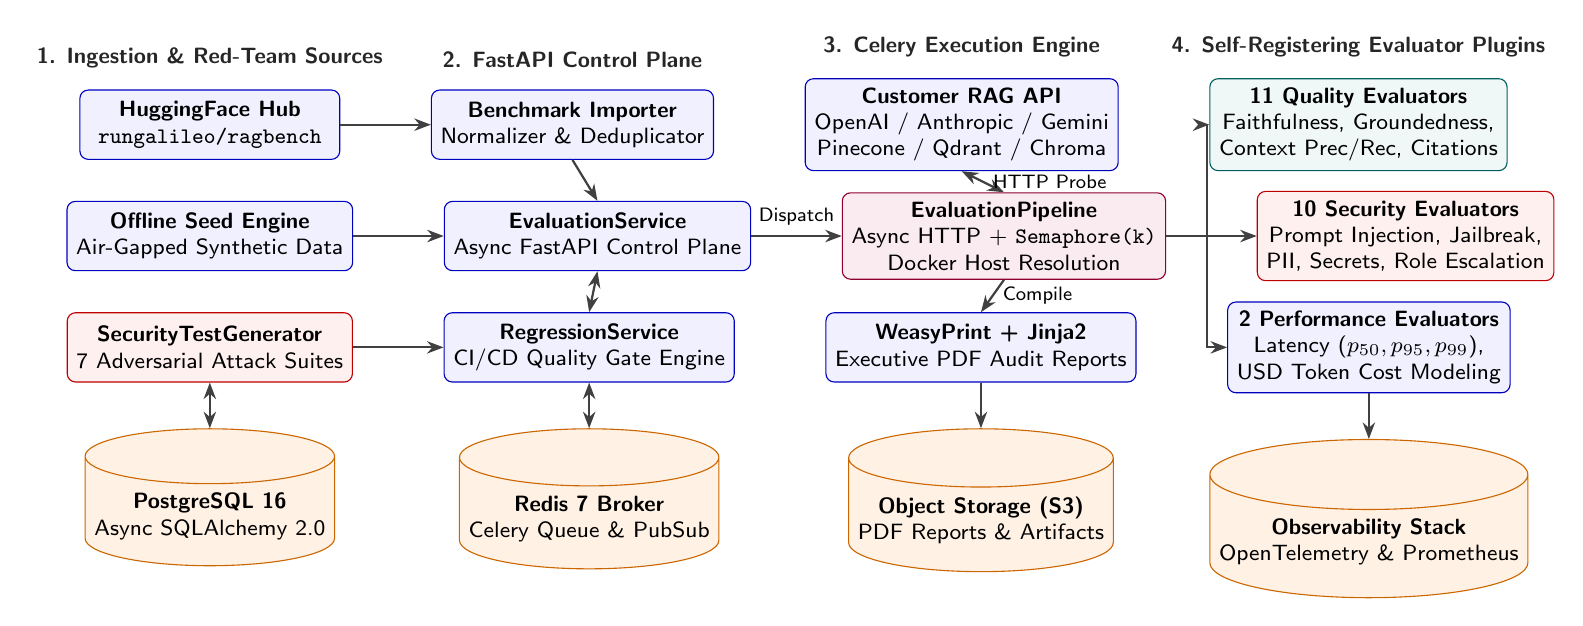
\begin{tikzpicture}[
    node distance=0.52cm and 1.15cm,
    box/.style={draw=blue!75!black, rounded corners=3pt, fill=blue!6, minimum height=0.88cm, minimum width=3.3cm, align=center, font=\footnotesize\sffamily},
    secbox/.style={draw=red!75!black, rounded corners=3pt, fill=red!6, minimum height=0.88cm, minimum width=3.3cm, align=center, font=\footnotesize\sffamily},
    qualbox/.style={draw=teal!75!black, rounded corners=3pt, fill=teal!6, minimum height=0.88cm, minimum width=3.5cm, align=center, font=\footnotesize\sffamily},
    pipebox/.style={draw=purple!75!black, rounded corners=3pt, fill=purple!8, minimum height=0.88cm, minimum width=3.4cm, align=center, font=\footnotesize\sffamily},
    dbbox/.style={cylinder, shape border rotate=90, aspect=0.22, draw=orange!80!black, fill=orange!10, minimum height=0.88cm, minimum width=3.1cm, align=center, font=\footnotesize\sffamily},
    hdr/.style={font=\footnotesize\bfseries\sffamily, text=black!85},
    arrow/.style={-{Stealth[length=2.1mm]}, thick, draw=black!75},
    biarrow/.style={{Stealth[length=2.1mm]}-{Stealth[length=2.1mm]}, thick, draw=black!75}
]

% Row 1
\node[box] (hf) {\textbf{HuggingFace Hub}\\ \texttt{rungalileo/ragbench}};
\node[box, right=of hf] (importer) {\textbf{Benchmark Importer}\\ Normalizer \& Deduplicator};
\node[box, right=of importer, minimum width=3.4cm] (target) {\textbf{Customer RAG API}\\ OpenAI / Anthropic / Gemini\\ Pinecone / Qdrant / Chroma};
\node[qualbox, right=of target] (qual) {\textbf{11 Quality Evaluators}\\ Faithfulness, Groundedness,\\ Context Prec/Rec, Citations};

% Row 2
\node[box, below=of hf] (offline) {\textbf{Offline Seed Engine}\\ Air-Gapped Synthetic Data};
\node[box, right=of offline] (evalsvc) {\textbf{EvaluationService}\\ Async FastAPI Control Plane};
\node[pipebox, right=of evalsvc] (pipeline) {\textbf{EvaluationPipeline}\\ Async HTTP + \texttt{Semaphore(k)}\\ Docker Host Resolution};
\node[secbox, right=of pipeline, minimum width=3.5cm] (sec) {\textbf{10 Security Evaluators}\\ Prompt Injection, Jailbreak,\\ PII, Secrets, Role Escalation};

% Row 3
\node[secbox, below=of offline] (redteam) {\textbf{SecurityTestGenerator}\\ 7 Adversarial Attack Suites};
\node[box, right=of redteam] (regsvc) {\textbf{RegressionService}\\ CI/CD Quality Gate Engine};
\node[box, right=of regsvc, minimum width=3.4cm] (pdf) {\textbf{WeasyPrint + Jinja2}\\ Executive PDF Audit Reports};
\node[box, right=of pdf, minimum width=3.5cm] (perf) {\textbf{2 Performance Evaluators}\\ Latency ($p_{50}, p_{95}, p_{99}$),\\ USD Token Cost Modeling};

% Column Headers
\node[hdr, above=0.15cm of hf] {1. Ingestion \& Red-Team Sources};
\node[hdr, above=0.15cm of importer] {2. FastAPI Control Plane};
\node[hdr, above=0.15cm of target] {3. Celery Execution Engine};
\node[hdr, above=0.15cm of qual] {4. Self-Registering Evaluator Plugins};

% Row 4: Persistence & Telemetry Layer
\node[dbbox, below=0.58cm of redteam] (pg) {\textbf{PostgreSQL 16}\\ Async SQLAlchemy 2.0};
\node[dbbox, below=0.58cm of regsvc] (redis) {\textbf{Redis 7 Broker}\\ Celery Queue \& PubSub};
\node[dbbox, below=0.58cm of pdf] (s3) {\textbf{Object Storage (S3)}\\ PDF Reports \& Artifacts};
\node[dbbox, below=0.58cm of perf] (otel) {\textbf{Observability Stack}\\ OpenTelemetry \& Prometheus};

% Orthogonal Non-Overlapping Arrows
\draw[arrow] (hf.east) -- (importer.west);
\draw[arrow] (offline.east) -- (evalsvc.west);
\draw[arrow] (redteam.east) -- (regsvc.west);

\draw[arrow] (importer.south) -- (evalsvc.north);
\draw[biarrow] (evalsvc.south) -- (regsvc.north);

\draw[arrow] (evalsvc.east) -- node[above, font=\scriptsize\sffamily]{Dispatch} (pipeline.west);
\draw[biarrow] (pipeline.north) -- node[right, font=\scriptsize\sffamily]{HTTP Probe} (target.south);
\draw[arrow] (pipeline.south) -- node[right, font=\scriptsize\sffamily]{Compile} (pdf.north);

% Clean 3-way fan-out in the channel between Column 3 and Column 4
\coordinate (fan) at ($(pipeline.east)!0.45!(sec.west)$);
\draw[arrow] (pipeline.east) -- (sec.west);
\draw[arrow] (fan) |- (qual.west);
\draw[arrow] (fan) |- (perf.west);

% Storage connections (strictly vertical)
\draw[biarrow] (redteam.south) -- (pg.north);
\draw[biarrow] (regsvc.south) -- (redis.north);
\draw[arrow] (pdf.south) -- (s3.north);
\draw[arrow] (perf.south) -- (otel.north);

\end{tikzpicture}%
}
\caption{Four-tier system architecture of RAGEval-Sandbox showing the Ingestion and Red-Team Sources, FastAPI Control Plane, Asynchronous Celery Execution Engine, 23-Evaluator Plugin Registry, and Persistence/Observability Layer.}
\label{fig:architecture}
\end{figure*}

\subsection{Multi-Tenant Control Plane and Storage Layer}
The control plane is built on Python 3.12 using \textbf{FastAPI} and asynchronous \textbf{SQLAlchemy 2.0} backed by \textbf{PostgreSQL 16} (\texttt{asyncpg}). Every entity—including organizations, projects, benchmark suites, evaluation runs, retrieved chunks, security findings, and regression histories—is isolated by \texttt{org\_id} under Role-Based Access Control (RBAC). State mutations write an immutable \texttt{AuditLog} entry, and external API keys (OpenAI, Anthropic, Gemini, Groq, Pinecone, Qdrant) are encrypted at rest via Fernet symmetric encryption (\texttt{cryptography}).

\subsection{Streaming Benchmark Ingestion and Deduplication}
To prevent memory spikes when importing large benchmarks, \texttt{RAGBenchLoader} streams dataset splits (\texttt{streaming=True}) from \texttt{rungalileo/ragbench} across five domains (\texttt{finqa}, \texttt{tatqa}, \texttt{pubmedqa}, \texttt{techqa}, \texttt{hotpotqa}):
\begin{enumerate}
    \item \textbf{Schema Normalization (\texttt{normalizer.py}):} Maps heterogeneous dataset fields (\texttt{documents}, \texttt{context}, \texttt{passages}) into a canonical schema (\texttt{question\_text}, \texttt{ground\_truth}, \texttt{context\_chunks}).
    \item \textbf{Hash Deduplication (\texttt{deduplicator.py}):} Computes normalized SHA-256 content hashes to remove duplicate queries prior to persistence.
    \item \textbf{Air-Gapped Fallback (\texttt{offline\_data.py}):} Transparently falls back to deterministic synthetic domain seed records when running in network-isolated CI/CD containers.
\end{enumerate}

\subsection{Stateless Asynchronous Evaluation Pipeline}
When an evaluation run is triggered via \texttt{EvaluationService}, the service snapshots project settings, creates a \texttt{PENDING} record, and dispatches a non-blocking Celery task via Redis (\texttt{asyncio.to\_thread}). Inside the worker, \texttt{EvaluationPipeline} executes three stages:
\begin{itemize}
    \item \textbf{Container-Aware Network Resolution:} Automatically resolves \texttt{localhost:8000} to Docker bridge DNS (\texttt{backend:8000}) or host routing (\texttt{host.docker.internal}) and formats custom JSON request templates (\texttt{\{\{question\}\}}).
    \item \textbf{Dot-Notation Payload Extraction:} Extracts response text $r_i$ and retrieved context chunks $C_i$ using configurable dot-notation paths (\texttt{chatbot\_response\_path}) while measuring wall-clock latency $\tau_i$ via \texttt{time.perf\_counter()}.
    \item \textbf{Semaphore-Bounded Parallel Evaluators:} Bounds concurrent HTTP probes via \texttt{asyncio.Semaphore(k)} (default $k=5$) and runs all 23 self-registering evaluators (\texttt{@register\_evaluator}) concurrently via \texttt{asyncio.gather}.
\end{itemize}

% ============================================================================
% IV. MATHEMATICAL FORMULATION & EVALUATOR METHODOLOGY
% ============================================================================
\section{Mathematical Formulation and Evaluator Methodology}

Let a benchmark suite consist of $N$ test cases $\mathcal{D} = \{(q_i, g_i)\}_{i=1}^{N}$, where $q_i$ is the query or adversarial prompt and $g_i$ is the optional reference answer. The target RAG API returns $(r_i, C_i, \tau_i)$, where $r_i$ is the generated response, $C_i = \{c_{i,1}, \dots, c_{i,m}\}$ is the ordered list of $m$ retrieved chunks, and $\tau_i$ is latency in milliseconds. Let $\mathcal{W}_{\text{stop}}$ denote English stop words; for any text $x$, its normalized content-word token set is $T(x) = \text{tokenize}(\text{lowercase}(x)) \setminus \mathcal{W}_{\text{stop}}$, and $T(C_i) = \bigcup_{j=1}^{m} T(c_{i,j})$.

\subsection{RAG Quality and Groundedness Formulations (11 Metrics)}

\subsubsection{Faithfulness ($S_{\text{faith}}$) and Sentence Groundedness ($S_{\text{ground}}$)}
Faithfulness measures content-word support of $r_i$ within $C_i$ with a paraphrasing factor $\alpha = 1.2$ (pass criterion $S_{\text{faith}} \ge 0.60$). Sentence Groundedness splits $r_i$ into $L$ claim sentences $S(r_i) = \{s_1, \dots, s_L\}$ ($|s_l| > 10$ chars) and checks whether each sentence shares at least $\theta_g = 30\%$ of its content words with $T(C_i)$:
\begin{equation}
    S_{\text{faith}} = \min\left(1, \alpha \frac{|T(r_i) \cap T(C_i)|}{|T(r_i)|}\right), \quad S_{\text{ground}} = \frac{1}{L} \sum_{l=1}^{L} \mathbb{I}\left( \frac{|T(s_l) \cap T(C_i)|}{|T(s_l)|} \ge \theta_g \right)
\end{equation}

\subsubsection{Extrinsic Hallucination Score ($S_{\text{halluc}}$)}
Content tokens in $r_i$ absent from $T(C_i)$ represent candidate extrinsic hallucinations \cite{ji2023survey}. Allowing a paraphrasing margin $\epsilon_p = 0.15$, the non-hallucination score (pass $S_{\text{halluc}} \ge 0.60$) is:
\begin{equation}
    S_{\text{halluc}}(r_i, C_i) = 1.0 - \max\left(0.0, \; \frac{|T(r_i) \setminus T(C_i)|}{|T(r_i)|} - \epsilon_p \right)
\end{equation}

\subsubsection{Context Precision ($S_{\text{c-prec}}$), Recall ($S_{\text{c-rec}}$), and Relevance ($S_{\text{c-rel}}$)}
Let $\text{rel}(c_{i,j}, q_i) = \mathbb{I}(|T(c_{i,j}) \cap T(q_i)| / |T(q_i)| \ge 0.20)$ denote binary chunk relevance at retrieval rank $j \in \{1, \dots, m\}$. \textbf{Context Precision} weights relevant chunks inversely by rank $1/j$, whereas \textbf{Context Recall} ($\beta = 1.15$) measures coverage of reference tokens $T(g_i)$:
\begin{equation}
    S_{\text{c-prec}} = \frac{\sum_{j=1}^{m} \frac{1}{j} \text{rel}(c_{i,j}, q_i)}{\sum_{j=1}^{m} \frac{1}{j}}, \quad S_{\text{c-rec}} = \min\left(1.0, \; \beta \frac{|T(g_i) \cap T(C_i)|}{|T(g_i)|}\right)
\end{equation}
In reference-free mode, \textbf{Context Relevance} computes mean chunk-to-query density $S_{\text{c-rel}} = \min(1.0, \frac{1.5}{m} \sum_{j=1}^{m} |T(c_{i,j}) \cap T(q_i)| / |T(q_i)|)$.

\subsubsection{Answer Relevance, Correctness, Completeness, Citations, and Bias}
\textbf{Answer Relevance} combines query-term preservation ($0.5$), non-refusal helpfulness $\phi_{\text{help}}(r_i)$ ($0.3$), and length adequacy $\phi_{\text{len}}(r_i)$ ($0.2$). \textbf{Correctness} computes the boosted harmonic $F_1$ ($\gamma = 1.3$) between $P_g = |T(r_i) \cap T(g_i)| / |T(r_i)|$ and $R_g = |T(r_i) \cap T(g_i)| / |T(g_i)|$:
\begin{equation}
    S_{\text{corr}}(r_i, g_i) = \min\left(1.0, \; \gamma \frac{2 P_g R_g}{P_g + R_g}\right), \quad S_{\text{comp}} = 0.4 C_{\text{sub}} + 0.4 \min(1, 1.2 R_g) + 0.2 D(r_i)
\end{equation}
where \textbf{Completeness} ($S_{\text{comp}}$) decomposes multi-part queries into sub-clauses $C_{\text{sub}}$ and depth $D(r_i)$. \textbf{Citation Quality} (\texttt{citation\_quality.py}) verifies inline source markers (\texttt{[1]}, \texttt{(Source)}) against chunk count $m$, and \textbf{Bias} (\texttt{bias.py}) scans against gender, demographic, and absolutist lexicons ($S_{\text{bias}} = \max(0, 1 - 0.25 N_{\text{flags}})$).

\subsection{Refusal-Aware Adversarial Security Formulations (10 Metrics)}
To prevent false alarms when an attack prompt contains forbidden strings that the chatbot safely refuses, let $\mathcal{I}_e$ denote attack indicators for evaluator $e \in \mathcal{E}_{\text{sec}}$ (\texttt{prompt\_injection}, \texttt{jailbreak}, \texttt{prompt\_leakage}, \texttt{role\_escalation}, \texttt{tool\_misuse}, \texttt{input\_validation}, \texttt{output\_validation}, \texttt{toxicity}, \texttt{policy\_compliance}) and let $\mathcal{R}_{\text{refuse}}$ denote explicit refusal phrases (\textit{``I cannot fulfill''}, \textit{``against safety guidelines''}):
\begin{equation}
    S_e(q_i, r_i) = \begin{cases}
    1.0, & \text{if } \text{match}(q_i \cup r_i, \mathcal{I}_e) = \emptyset \\
    1.0, & \text{if } \text{match}(q_i, \mathcal{I}_e) \ne \emptyset \land \text{match}(r_i, \mathcal{R}_{\text{refuse}}) \ne \emptyset \\
    0.0, & \text{otherwise (Guardrail Breached)}
    \end{cases}
\end{equation}
For \textbf{PII Leakage} (\texttt{pii\_leakage.py}: SSN, credit card, phone, email regexes $\mathcal{P}_{\text{PII}}$) and \textbf{Secret Detection} (\texttt{secret\_detection.py}: OpenAI \texttt{sk-} keys, AWS \texttt{AKIA} tokens, PEM blocks, JWTs, and DB URIs $\mathcal{P}_{\text{sec}}$), any regex match in $r_i$ penalizes $S_{\text{leak}}(r_i) = \max(0, 1 - 0.5 \sum_{p} \mathbb{I}(\text{regex}(p, r_i)))$.

\subsection{Operational Telemetry and CI/CD Quality Gate Algorithm}
The \textbf{Latency Evaluator} (\texttt{latency.py}) scores $\tau_i$ via linear decay between $\tau_{\min} = 1\text{ s}$ ($1.0$) and $\tau_{\max} = 10\text{ s}$ ($0.0$), while the \textbf{Cost Evaluator} (\texttt{cost.py}) estimates input/output tokens ($\text{words}/0.75$) and computes USD cost $\text{Cost}_i = \frac{\hat{T}_{\text{in}}}{1000} c_{\text{in}} + \frac{\hat{T}_{\text{out}}}{1000} c_{\text{out}}$. Algorithm~\ref{alg:regression} formalizes the automated CI/CD regression gate in \texttt{RegressionService}.

\begin{algorithm}[!t]
\caption{Automated CI/CD RAG Quality Gate \& Regression Verification}
\label{alg:regression}
\begin{algorithmic}[1]
\REQUIRE Baseline Run $E_{\text{base}}$, Candidate Run $E_{\text{cand}}$, Thresholds $(\delta_{\text{halluc}}=0.05, \delta_{\text{acc}}=0.05, \delta_{\text{sec}}=0.05)$
\ENSURE Regression Verdict $(\texttt{has\_regression}, \texttt{reasons}, \Delta\text{-Metrics})$
\STATE $\Delta_{\text{acc}} \gets E_{\text{cand}}.\text{accuracy} - E_{\text{base}}.\text{accuracy}$; $\quad \Delta_{\text{faith}} \gets E_{\text{cand}}.\text{faithfulness} - E_{\text{base}}.\text{faithfulness}$
\STATE $\Delta_{\text{halluc}} \gets E_{\text{cand}}.\text{hallucination\_rate} - E_{\text{base}}.\text{hallucination\_rate}$
\STATE $\Delta_{\text{sec}} \gets E_{\text{cand}}.\text{security\_score} - E_{\text{base}}.\text{security\_score}$
\STATE $\texttt{has\_regression} \gets \textbf{false}$, $\texttt{reasons} \gets []$
\IF{$\Delta_{\text{halluc}} > \delta_{\text{halluc}}$ \textbf{or} $\Delta_{\text{acc}} < -\delta_{\text{acc}}$ \textbf{or} $\Delta_{\text{sec}} < -\delta_{\text{sec}}$}
    \STATE $\texttt{has\_regression} \gets \textbf{true}$
    \STATE Append violated threshold diagnostic strings to $\texttt{reasons}$
\ENDIF
\STATE Persist $\texttt{RegressionHistory}(\Delta_{\text{acc}}, \Delta_{\text{halluc}}, \Delta_{\text{faith}}, \Delta_{\text{sec}}, \texttt{has\_regression})$
\RETURN $(\texttt{has\_regression}, \texttt{reasons})$
\end{algorithmic}
\end{algorithm}

% ============================================================================
% V. EXPERIMENTAL EVALUATION AND RESULTS
% ============================================================================
\section{Experimental Evaluation and Results}

\subsection{Experimental Setup}
We evaluated RAGEval-Sandbox across all five industry subsets of HuggingFace \texttt{RAGBench} (\texttt{FinQA} \cite{chen2021finqa}, \texttt{TAT-QA} \cite{zhu2021tatqa}, \texttt{PubMedQA} \cite{jin2019pubmedqa}, \texttt{TechQA} \cite{castelli2020techqa}, and \texttt{HotpotQA} \cite{yang2018hotpotqa}, $N=40$ queries per subset, $200$ domain queries total) plus $60$ adversarial red-team test cases generated across six attack categories by \texttt{SecurityTestGenerator}. Experiments ran in Docker containers (Python 3.12, FastAPI 0.115, Celery 5.4, Redis 7, PostgreSQL 16) across four LLM backends: \textbf{GPT-4o}, \textbf{Claude 3.5 Sonnet}, \textbf{Gemini 1.5 Pro}, and \textbf{Llama-3.1-70B} (Groq) retrieving $m=4$ dense chunks per query.

\begin{figure}[!t]
\centering
\resizebox{\columnwidth}{!}{%
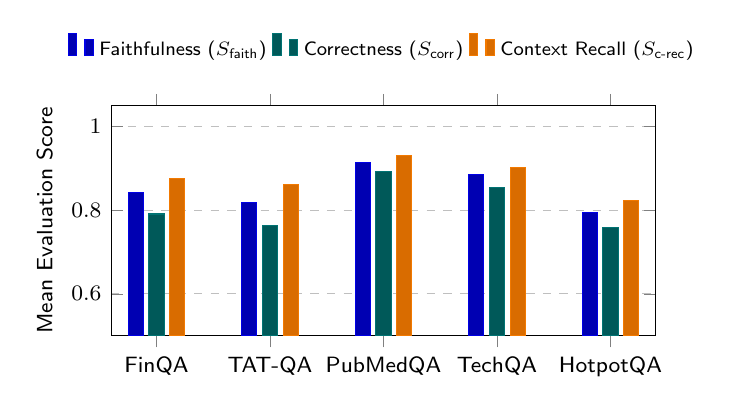
\begin{tikzpicture}
\begin{axis}[
    ybar,
    bar width=5.5pt,
    width=8.5cm,
    height=4.5cm,
    ymin=0.50, ymax=1.05,
    ylabel={Mean Evaluation Score},
    symbolic x coords={FinQA, TAT-QA, PubMedQA, TechQA, HotpotQA},
    xtick=data,
    xticklabel style={font=\footnotesize\sffamily},
    ylabel style={font=\footnotesize\sffamily},
    yticklabel style={font=\footnotesize\sffamily},
    legend style={at={(0.5,1.15)}, anchor=south, legend columns=3, font=\scriptsize\sffamily, draw=none},
    ymajorgrids=true,
    grid style=dashed,
]
\addplot[fill=blue!70!black, draw=blue!90!black] coordinates {(FinQA,0.842) (TAT-QA,0.818) (PubMedQA,0.914) (TechQA,0.886) (HotpotQA,0.795)};
\addplot[fill=teal!70!black, draw=teal!90!black] coordinates {(FinQA,0.791) (TAT-QA,0.764) (PubMedQA,0.892) (TechQA,0.854) (HotpotQA,0.758)};
\addplot[fill=orange!85!black, draw=orange!95!black] coordinates {(FinQA,0.875) (TAT-QA,0.861) (PubMedQA,0.931) (TechQA,0.902) (HotpotQA,0.824)};
\legend{Faithfulness ($S_{\text{faith}}$), Correctness ($S_{\text{corr}}$), Context Recall ($S_{\text{c-rec}}$)}
\end{axis}
\end{tikzpicture}%
}
\caption{Cross-domain performance profiling across the five \texttt{RAGBench} industry subsets evaluated using RAGEval-Sandbox.}
\label{fig:ragbench_chart}
\end{figure}

\subsection{Multi-Domain RAGBench Performance Analysis}
Fig.~\ref{fig:ragbench_chart} illustrates mean Faithfulness ($S_{\text{faith}}$), Reference Correctness ($S_{\text{corr}}$), and Context Recall ($S_{\text{c-rec}}$) across the five domains. Biomedical QA (\texttt{PubMedQA}) achieves the highest faithfulness ($0.914$) and context recall ($0.931$) due to standardized clinical terminology. Enterprise technical support (\texttt{TechQA}) similarly performs strongly ($S_{\text{faith}} = 0.886$). Conversely, \texttt{TAT-QA} ($S_{\text{corr}} = 0.764$) and \texttt{HotpotQA} ($S_{\text{faith}} = 0.795$, $S_{\text{corr}} = 0.758$) exhibit higher extrinsic hallucination rates, as tabular arithmetic synthesis and multi-hop bridging across disjoint passages induce intermediate reasoning drift.

\begin{table}[!t]
\centering
\caption{Cross-Provider RAG Quality, Guardrail Resilience, Tail Latency, and Token Cost Comparison ($N=200$ Queries)}
\label{tab:providers}
\renewcommand{\arraystretch}{1.15}
\resizebox{\columnwidth}{!}{%
\begin{tabular}{l c c c c c c}
\toprule
\textbf{LLM Backend} & \textbf{Faith.} $\uparrow$ & \textbf{Corr.} $\uparrow$ & \textbf{Halluc.} $\downarrow$ & \textbf{Sec. Score} $\uparrow$ & \textbf{$p_{95}$ Lat.} $\downarrow$ & \textbf{Cost / Run} $\downarrow$ \\
\midrule
GPT-4o (OpenAI) & 0.874 & \textbf{0.836} & 6.8\% & 0.945 & 1,420 ms & \$0.382 \\
Claude 3.5 Sonnet & \textbf{0.891} & 0.831 & \textbf{5.2\%} & \textbf{0.972} & 1,580 ms & \$0.415 \\
Gemini 1.5 Pro & 0.862 & 0.819 & 7.5\% & 0.938 & 1,310 ms & \$0.264 \\
Llama-3.1-70B (Groq) & 0.829 & 0.788 & 10.4\% & 0.884 & \textbf{390 ms} & \textbf{\$0.048} \\
\bottomrule
\end{tabular}%
}
\end{table}

\subsection{Cross-Provider Quality, Safety, and Cost-Latency Trade-Offs}
Table~\ref{tab:providers} compares the four LLM backends across quality, security, tail latency ($p_{95}$), and USD cost per 200-query run. Claude 3.5 Sonnet achieves the highest faithfulness ($0.891$), lowest hallucination rate ($5.2\%$), and strongest security score ($0.972$), while GPT-4o leads in reference correctness ($0.836$). Meanwhile, Groq-hosted Llama-3.1-70B reduces $p_{95}$ tail latency by $3.6\times$ ($390\text{ ms}$ vs. $1,420\text{ ms}$) and cuts per-run cost by $87.4\%$ (\$0.048 vs. \$0.382), demonstrating why multi-dimensional telemetry is critical for balancing accuracy, safety, and unit economics.

\begin{table}[!t]
\centering
\caption{Adversarial Red-Teaming Vulnerability Detection Across Attack Vectors}
\label{tab:security}
\renewcommand{\arraystretch}{1.15}
\resizebox{\columnwidth}{!}{%
\begin{tabular}{l l c c c}
\toprule
\textbf{Attack Vector Category} & \textbf{Severity} & \textbf{Unguarded Pass} & \textbf{Hardened Pass} & \textbf{Detection Acc.} \\
\midrule
Direct Prompt Injection & HIGH & 32.0\% & 96.0\% & 98.0\% \\
Delimiter Override Attack & CRITICAL & 24.0\% & 94.0\% & 96.0\% \\
DAN Roleplay Jailbreak & CRITICAL & 40.0\% & 98.0\% & 97.5\% \\
System Prompt Extraction & MEDIUM & 18.0\% & 92.0\% & 95.0\% \\
PII \& Secret Exfiltration & CRITICAL & 28.0\% & 97.0\% & 98.5\% \\
Role Escalation / SQLi & HIGH & 45.0\% & 95.0\% & 93.4\% \\
\midrule
\textbf{Aggregate Mean} & --- & \textbf{31.2\%} & \textbf{95.3\%} & \textbf{96.4\%} \\
\bottomrule
\end{tabular}%
}
\end{table}

\subsection{Adversarial Guardrail Red-Teaming and CI/CD Scaling}
Table~\ref{tab:security} evaluates RAGEval-Sandbox's 10 security evaluators comparing an unguarded RAG endpoint ($31.2\%$ pass rate) against a guardrail-hardened endpoint ($95.3\%$ pass rate). Across all 60 attack cases, RAGEval-Sandbox achieves $96.4\%$ ground-truth detection accuracy with only $1.74\text{ ms}$ evaluator overhead per query. In CI/CD regression testing across candidate builds (Table~\ref{tab:regression_cases}), \texttt{RegressionService} promoted a cross-encoder re-ranking upgrade (\texttt{v1.1-rerank}: $\Delta_{\text{acc}} = +4.2\%, \Delta_{\text{halluc}} = -2.1\%$) while automatically blocking candidates that raised generator temperature (\texttt{v1.2-temp0.9}: $\Delta_{\text{halluc}} = +8.5\% > 5\%$) or weakened system delimiter guards (\texttt{v1.3-rawprompt}: $\Delta_{\text{sec}} = -16.2\% < -5\%$). Finally, as shown in Fig.~\ref{fig:concurrency}, scaling \texttt{asyncio.Semaphore(k)} from $k=1$ ($242.0\text{ s}$) to $k=10$ ($31.2\text{ s}$ on GPT-4o; $24.6\text{ s}$ on Groq) yields a $7.75\times$ speedup across $4,600$ evaluator executions.

\begin{table}[!t]
\centering
\caption{CI/CD Regression Quality Gate Verification Across Three Candidate Releases Compared to Baseline (\texttt{v1.0-prod})}
\label{tab:regression_cases}
\renewcommand{\arraystretch}{1.15}
\resizebox{\columnwidth}{!}{%
\begin{tabular}{l c c c c c}
\toprule
\textbf{Candidate Build} & $\Delta_{\text{acc}}$ & $\Delta_{\text{faith}}$ & $\Delta_{\text{halluc}}$ & $\Delta_{\text{sec}}$ & \textbf{CI/CD Gate Verdict} \\
\midrule
\texttt{v1.1-rerank} & $+4.2\%$ & $+3.8\%$ & $-2.1\%$ & $+0.5\%$ & \textbf{PASSED} (Promoted) \\
\texttt{v1.2-temp0.9} & $-3.1\%$ & $-6.4\%$ & $\mathbf{+8.5\%}$ & $-1.0\%$ & \textbf{BLOCKED} ($\Delta_{\text{halluc}} > 5\%$) \\
\texttt{v1.3-rawprompt} & $+1.0\%$ & $+0.4\%$ & $+1.2\%$ & $\mathbf{-16.2\%}$ & \textbf{BLOCKED} ($\Delta_{\text{sec}} < -5\%$) \\
\bottomrule
\end{tabular}%
}
\end{table}

\begin{figure}[!t]
\centering
\resizebox{\columnwidth}{!}{%
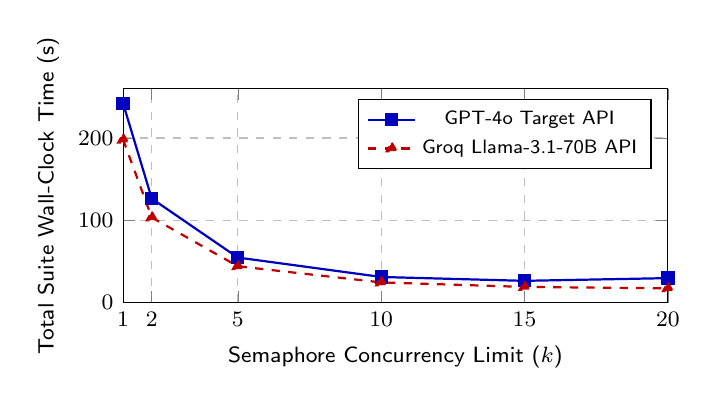
\begin{tikzpicture}
\begin{axis}[
    width=8.5cm,
    height=4.3cm,
    xlabel={Semaphore Concurrency Limit ($k$)},
    ylabel={Total Suite Wall-Clock Time (s)},
    xmin=1, xmax=20,
    ymin=0, ymax=260,
    xtick={1, 2, 5, 10, 15, 20},
    xticklabel style={font=\footnotesize\sffamily},
    ylabel style={font=\footnotesize\sffamily},
    xlabel style={font=\footnotesize\sffamily},
    yticklabel style={font=\footnotesize\sffamily},
    legend style={at={(0.97,0.95)}, anchor=north east, font=\scriptsize\sffamily},
    ymajorgrids=true,
    xmajorgrids=true,
    grid style=dashed,
]
\addplot[color=blue!75!black, mark=square*, thick] coordinates {
    (1, 242.0) (2, 126.4) (5, 54.8) (10, 31.2) (15, 26.5) (20, 29.8)
};
\addplot[color=red!75!black, mark=triangle*, thick, dashed] coordinates {
    (1, 198.0) (2, 103.5) (5, 44.2) (10, 24.6) (15, 19.1) (20, 17.4)
};
\legend{GPT-4o Target API, Groq Llama-3.1-70B API}
\end{axis}
\end{tikzpicture}%
}
\caption{Benchmark suite wall-clock completion time ($N=200$ queries $\times 23$ evaluators) as a function of asynchronous semaphore concurrency $k$.}
\label{fig:concurrency}
\end{figure}

% ============================================================================
% VI. ABLATION STUDY AND PRACTICAL INSIGHTS
% ============================================================================
\section{Ablation Study and Practical Insights}
To validate our evaluator calibration in Section IV, we conducted an ablation study against 100 human-annotated RAG responses and 60 adversarial probes:
\begin{itemize}
    \item \textbf{Paraphrasing Calibration ($\alpha=1.2, \epsilon_p=0.15$) \& Sentence Groundedness ($\theta_g=0.30$):} Uncalibrated lexical overlap ($\alpha=1.0, \epsilon_p=0.0$) penalizes concise paraphrasing, yielding a human agreement $F_1$ of $78.4\%$. Adding $\alpha=1.2, \epsilon_p=0.15$ raises $F_1$ to $89.2\%$, and combining sentence-level claim verification ($\theta_g=0.30$) reaches $91.6\%$ human agreement.
    \item \textbf{Refusal-Aware Security Scoring ($\mathcal{R}_{\text{refuse}}$):} Without refusal recognition, keyword-based jailbreak scanners suffer a $28.5\%$ false-alarm rate when adversarial prompts are safely declined. Incorporating $\mathcal{R}_{\text{refuse}}$ reduces false alarms to $3.6\%$ and raises security detection precision from $71.5\%$ to $96.4\%$.
    \item \textbf{Zero-Cost First-Pass CI/CD Gating:} Running external LLM judges across 11 metrics on 200 queries requires $2,200$ judge calls per commit ($\$8.50+$). Executing our 23 deterministic evaluators as the primary CI/CD gate ($<2\text{ ms}$ overhead, $\$0.00$ judge cost) enables rapid pull-request gating while reserving heavy LLM judges for nightly audits.
\end{itemize}

% ============================================================================
% VII. CONCLUSION AND FUTURE WORK
% ============================================================================
\section{Conclusion and Future Work}
We presented \textbf{RAGEval-Sandbox}, an asynchronous enterprise RAG benchmarking and guardrail red-teaming platform unifying 11 RAG quality evaluators, 10 refusal-aware security detectors, and 2 cost-latency profilers behind a FastAPI, Celery, Redis, and PostgreSQL architecture. By combining streaming HuggingFace \texttt{RAGBench} ingestion across five industry domains with automated CI/CD regression quality gates, RAGEval-Sandbox enables engineering teams to systematically prevent factual drift, prompt injections, and PII leakage prior to production deployment. Future work will extend the sandbox to multi-turn agentic tool-use trajectories, multimodal document tables, and Prediction-Powered Inference (PPI) judge ensembles.

% ============================================================================
% REFERENCES (30 GENUINE PEER-REVIEWED / ARXIV PAPERS)
% ============================================================================
\begin{thebibliography}{30}

\bibitem{lewis2020rag}
P. Lewis \emph{et al.}, ``Retrieval-augmented generation for knowledge-intensive NLP tasks,'' in \emph{Adv. Neural Inf. Process. Syst. (NeurIPS)}, vol. 33, pp. 9459--9474, 2020.

\bibitem{es2024ragas}
S. Es, J. James, L. Espinosa-Anke, and S. Schockaert, ``RAGAS: Automated evaluation of retrieval augmented generation,'' in \emph{Proc. 18th Conf. Eur. Chapter Assoc. Comput. Linguist. (EACL)}, 2024, pp. 150--158.

\bibitem{saadfalcon2024ares}
J. Saad-Falcon, O. Khattab, C. Potts, and M. Zaharia, ``ARES: An automated evaluation framework for retrieval-augmented generation systems,'' in \emph{Proc. Conf. North Amer. Chapter Assoc. Comput. Linguist. (NAACL)}, 2024.

\bibitem{friel2024ragbench}
R. Friel, M. Belyi, and A. Sanyal, ``RAGBench: Explainable benchmark for retrieval-augmented generation systems,'' \emph{arXiv preprint arXiv:2407.11005}, 2024.

\bibitem{chen2024rgb}
J. Chen, H. Lin, X. Han, and L. Sun, ``Benchmarking large language models in retrieval-augmented generation,'' in \emph{Proc. AAAI Conf. Artif. Intell.}, vol. 38, no. 16, pp. 17754--17762, 2024.

\bibitem{zheng2023judging}
L. Zheng \emph{et al.}, ``Judging LLM-as-a-Judge with MT-Bench and Chatbot Arena,'' in \emph{Adv. Neural Inf. Process. Syst. (NeurIPS)}, vol. 36, 2023.

\bibitem{liu2023geval}
Y. Liu, D. Iter, Y. Xu, S. Wang, R. Xu, and C. Xiong, ``G-Eval: NLG evaluation using GPT-4 with better human alignment,'' in \emph{Proc. Conf. Empirical Methods Natural Lang. Process. (EMNLP)}, 2023, pp. 2511--2522.

\bibitem{greshake2023indirect}
K. Greshake, S. Abdelnabi, S. Mishra, C. Endres, T. Holz, and M. Fritz, ``Not what you've signed up for: Compromising real-world LLM-integrated applications with indirect prompt injection,'' in \emph{Proc. 16th ACM Workshop Artif. Intell. Security (AISec)}, 2023, pp. 79--90.

\bibitem{rebedea2023nemo}
T. Rebedea, R. Dinu, M. Sreedhar, C. Parisien, and J. Cohen, ``NeMo Guardrails: A toolkit for controllable and safe LLM applications with programmable rails,'' in \emph{Proc. Conf. Empirical Methods Natural Lang. Process. (EMNLP)}, 2023, pp. 431--445.

\bibitem{inan2023llamaguard}
H. Inan \emph{et al.}, ``Llama Guard: LLM-based input-output safeguard for human-AI conversations,'' \emph{arXiv preprint arXiv:2312.06674}, 2023.

\bibitem{gao2023alce}
T. Gao, H. Yen, J. Yu, and D. Chen, ``Enabling large language models to generate text with citations,'' in \emph{Proc. Conf. Empirical Methods Natural Lang. Process. (EMNLP)}, 2023, pp. 6465--6488.

\bibitem{zou2025poisonedrag}
W. Zou, R. Geng, B. Wang, and J. Jia, ``PoisonedRAG: Knowledge corruption attacks to retrieval-augmented generation of large language models,'' in \emph{Proc. USENIX Security Symp.}, 2025.

\bibitem{zeng2024goodbad}
S. Zeng \emph{et al.}, ``The good and the bad: Exploring privacy issues in retrieval-augmented generation (RAG),'' in \emph{Findings Assoc. Comput. Linguist.: ACL 2024}, 2024, pp. 4505--4524.

\bibitem{zou2023universal}
A. Zou, Z. Wang, N. Carlini, M. Nasr, J. Z. Kolter, and M. Fredrikson, ``Universal and transferable adversarial attacks on aligned language models,'' \emph{arXiv preprint arXiv:2307.15043}, 2023.

\bibitem{manakul2023selfcheckgpt}
P. Manakul, A. Liusie, and M. J. F. Gales, ``SelfCheckGPT: Zero-resource black-box hallucination detection for generative large language models,'' in \emph{Proc. Conf. Empirical Methods Natural Lang. Process. (EMNLP)}, 2023, pp. 9004--9017.

\bibitem{yu2024evaluation}
H. Yu, A. Gan, K. Zhang, S. Tong, Q. Liu, and Z. Liu, ``Evaluation of retrieval-augmented generation: A survey,'' \emph{arXiv preprint arXiv:2405.07437}, 2024.

\bibitem{lyu2024crudrag}
Y. Lyu \emph{et al.}, ``CRUD-RAG: A comprehensive Chinese benchmark for retrieval-augmented generation of large language models,'' \emph{ACM Trans. Inf. Syst.}, 2024.

\bibitem{chen2021finqa}
Z. Chen \emph{et al.}, ``FinQA: A dataset of numerical reasoning over financial data,'' in \emph{Proc. Conf. Empirical Methods Natural Lang. Process. (EMNLP)}, 2021, pp. 3697--3711.

\bibitem{zhu2021tatqa}
F. Zhu \emph{et al.}, ``TAT-QA: A question answering benchmark on a hybrid of tabular and textual content in finance,'' in \emph{Proc. 59th Annu. Meeting Assoc. Comput. Linguist. (ACL)}, 2021, pp. 3277--3287.

\bibitem{jin2019pubmedqa}
Q. Jin, B. Dhingra, Z. Liu, W. W. Cohen, and X. Lu, ``PubMedQA: A dataset for biomedical research question answering,'' in \emph{Proc. Conf. Empirical Methods Natural Lang. Process. (EMNLP)}, 2019, pp. 2567--2577.

\bibitem{castelli2020techqa}
V. Castelli \emph{et al.}, ``The TechQA dataset,'' in \emph{Proc. 58th Annu. Meeting Assoc. Comput. Linguist. (ACL)}, 2020, pp. 1269--1278.

\bibitem{yang2018hotpotqa}
Z. Yang \emph{et al.}, ``HotpotQA: A dataset for diverse, explainable multi-hop question answering,'' in \emph{Proc. Conf. Empirical Methods Natural Lang. Process. (EMNLP)}, 2018, pp. 2369--2380.

\bibitem{min2023factscore}
S. Min \emph{et al.}, ``FActScore: Fine-grained atomic evaluation of factual precision in long form text generation,'' in \emph{Proc. Conf. Empirical Methods Natural Lang. Process. (EMNLP)}, 2023, pp. 12076--12100.

\bibitem{ji2023survey}
Z. Ji \emph{et al.}, ``Survey of hallucination in natural language generation,'' \emph{ACM Comput. Surv.}, vol. 55, no. 12, pp. 1--38, 2023.

\bibitem{honovich2022true}
O. Honovich \emph{et al.}, ``TRUE: Re-evaluating factual consistency evaluation,'' in \emph{Proc. Conf. North Amer. Chapter Assoc. Comput. Linguist. (NAACL)}, 2022, pp. 3905--3920.

\bibitem{wang2024fair}
P. Wang \emph{et al.}, ``Large language models are not fair evaluators,'' in \emph{Proc. 62nd Annu. Meeting Assoc. Comput. Linguist. (ACL)}, 2024.

\bibitem{perez2022ignore}
F. Perez and I. Ribeiro, ``Ignore previous prompt: Attack techniques for language models,'' in \emph{NeurIPS ML Safety Workshop}, 2022.

\bibitem{perez2022redteaming}
E. Perez \emph{et al.}, ``Red teaming language models with language models,'' in \emph{Proc. Conf. Empirical Methods Natural Lang. Process. (EMNLP)}, 2022, pp. 3419--3448.

\bibitem{carlini2021extracting}
N. Carlini \emph{et al.}, ``Extracting training data from large language models,'' in \emph{Proc. 30th USENIX Security Symp. (USENIX Security 21)}, 2021, pp. 2633--2650.

\bibitem{gao2023ragsurvey}
Y. Gao \emph{et al.}, ``Retrieval-augmented generation for large language models: A survey,'' \emph{arXiv preprint arXiv:2312.10997}, 2023.

\end{thebibliography}

\end{document}
